\documentclass[11pt]{article}
\usepackage[utf8]{inputenc}
\usepackage{amsfonts}
\usepackage{natbib}
\usepackage{graphicx}
\usepackage{amsmath}
\usepackage{amssymb}
\usepackage{mathrsfs} % Cursive font
\usepackage{ragged2e}
\usepackage{fancyhdr}
\usepackage{nameref}
\usepackage{wrapfig}
\usepackage{hyperref}


% \usepackage[left=2cm, right=2cm, top=2cm,bottom=2cm]{geometry}


\usepackage{mathtools}
\usepackage{xparse} \DeclarePairedDelimiterX{\Iintv}[1]{\llbracket}{\rrbracket}{\iintvargs{#1}}
\NewDocumentCommand{\iintvargs}{>{\SplitArgument{1}{,}}m}
{\iintvargsaux#1}
\NewDocumentCommand{\iintvargsaux}{mm} {#1\mkern1.5mu,\mkern1.5mu#2}

\makeatletter
\newcommand*{\currentname}{\@currentlabelname}
\makeatother

% \usepackage[a4paper,hmargin=1in, vmargin=1.4in,footskip=0.25in]{geometry}

\graphicspath{ {./images/} }


%\addtolength{\hoffset}{-1cm}
%\addtolength{\hoffset}{-2.5cm}
%\addtolength{\voffset}{-2.5cm}
\addtolength{\textwidth}{0.2cm}
%\addtolength{\textheight}{2cm}
\setlength{\parskip}{8pt}
\setlength{\parindent}{0.5cm}
\linespread{1.5}

\pagestyle{fancy}
\fancyhf{}
\rhead{TP Ontologías - Cipullo, Sullivan}
\lhead{Introducción a la Inteligencia Artificial}
\rfoot{\vspace{1cm} \thepage}

\renewcommand*\contentsname{\LARGE Índice}

\setlength{\skip\footins}{0.5cm}

\begin{document}

\begin{titlepage}
    \hspace{-2.5cm}
\includegraphics[scale= 0.48]{header.png}
    \begin{center}
        \vfill
            \noindent\textbf{\Huge Introducción a la Inteligencia Artificial}\par
            \vspace{.5cm}
            \noindent\textbf{\Huge Trabajo Práctico Ontologías}\par
            \vspace{.5cm}
        \vfill
        \noindent \textbf{\huge Alumnas:}\par
        \vspace{.5cm}
        \noindent \textbf{\Large Cipullo, Inés}\par
        \noindent \textbf{\Large Sullivan, Katherine}\par
 
        \vfill
        % \large Universidad Nacional de Rosario \par
        \noindent\large 2022
    \end{center}
\end{titlepage}
\ 

\section{Descripción del dominio}
La ontología presentada busca representar el dominio geopolítico, entendiendo por geopolítica a la disciplina que estudia los efectos de la geografía humana y física sobre la política y las relaciones internacionales.

El principal objetivo de esta ontología es proporcionar un punto de referencia para la búsqueda de información sobre países y otros territorios, y su respectiva posición en la realidad internacional actual, centrándose principalmente en las relaciones entre los mismos. 

\section{Listado de conceptos}
\begin{itemize}
    \item Territorio: área incluyendo tierras, aguas y espacio aéreo. Delimitación geográfica en la cual se encuentra asentada una población.
    \begin{itemize}
        \item Continente: gran extensión de tierra que se diferencia de otras menores o sumergidas por conceptos geográficos, como son los océanos; culturales, como la etnografía; y la historia de cada uno.
        \item País: territorio con características geográficas y culturales propias que constituye un Estado soberano.
        \item Territorio dependiente: territorio que cuenta con cierto grado de autonomía pero que por diversas razones no goza de los privilegios de total independencia o soberanía, ni hace parte integral del Estado que lo gobierna.
    \end{itemize}
    \item Forma de gobierno: manera en la que se estructura el poder político para ejercer su autoridad en el Estado. 
    \begin{itemize}
        \item Gobierno republicano: forma de gobierno en la que el jefe del estado no es un monarca, sino un cargo público cuyo ocupante no tiene derecho por sí mismo a ejercerlo, sino que lo ha obtenido mediante un procedimiento de elección pública directa o indirecta. 
        \item Gobierno monárquico: forma de gobierno gobierno en la que la jefatura del estado es personal, vitalicia y designada a un monarca. 
        \item Gobierno por junta militar: sistema en el que el gobierno está formado exclusivamente por altos mandos de las fuerzas armadas de su Estado.
        \item Gobierno teocrático: forma de gobierno sin separación de poderes entre la autoridad política y la religiosa. Su cuerpo legislativo está supeditado a la legislación interna de la religión dominante.
    \end{itemize}
    \item Grupo: conjunto internacional organizado con un fin común.
    \begin{itemize}
        \item Organización no gubernamental: organizaciones que no son parte de las esferas gubernamentales o empresas, cuyo fin fundamental es el bien social.
        \item Grupo económico: agrupación de países con el propósito de obtener beneficios en el comercio internacional.
        \item Alianza militar: sistema de defensa colectiva, en el cual los Estados integrantes acuerdan defender a cualquiera de sus miembros que sea atacado por un externo. 
    \end{itemize}
    \item Armamento: conjunto de armas al servicio de un ejército. 
    \begin{itemize}
        \item Armamento nuclear: explosivos de alto poder que utilizan la energía nuclear y los vectores que la portan (misiles balísticos y bombarderos).
        \item Armamento aéreo: armamento utilizado en una aeronave, ya sea interno o externo, lanzable o no.
        \item Armamento naval: armamento utilizado en los buques de guerra para destruir barcos enemigos.
    \end{itemize}
\end{itemize}

\section{Diagrama de la ontología}

\hspace{-2cm}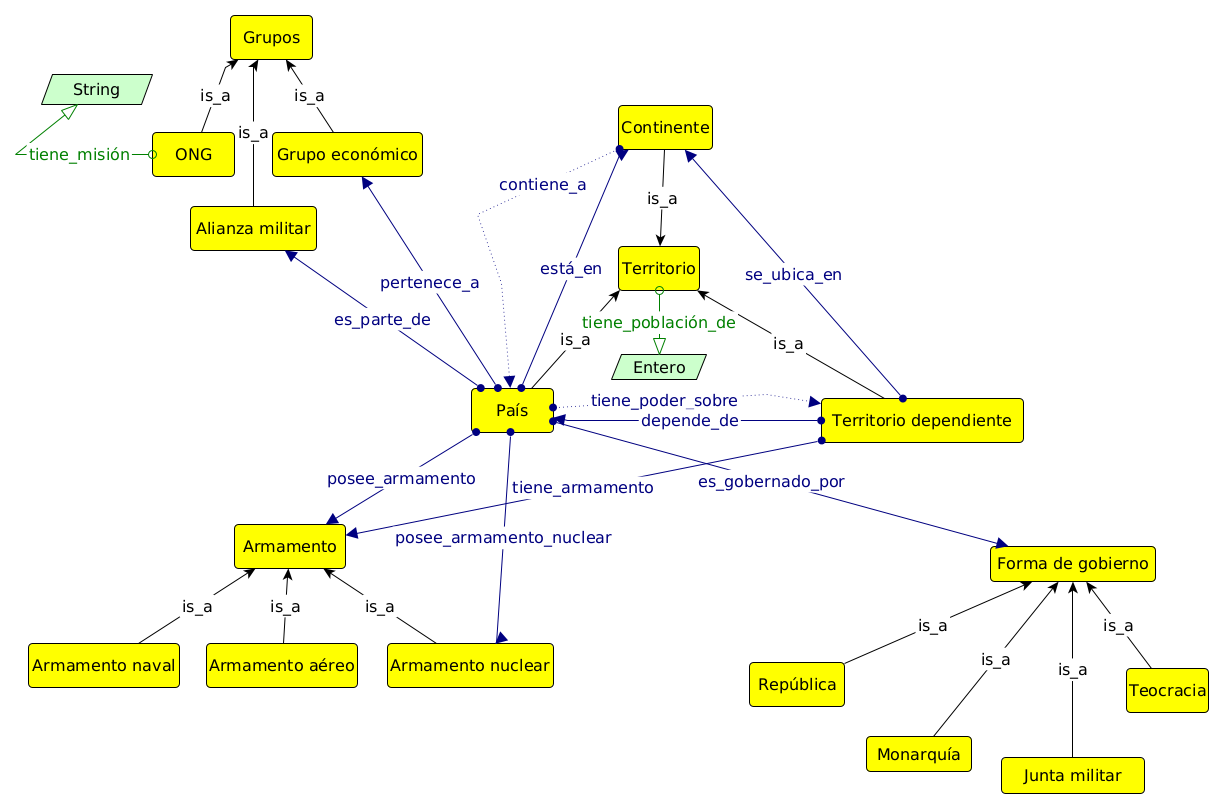
\includegraphics[scale=0.4]{ontologia.png}

\section{Instanciación}

Agregamos a nuestra ontología los continentes África, América, Asia (de quien definimos su población), Europa y Oceanía. 

Luego, los países Argentina (de quien explicitamos su población, su forma de gobierno y el continente y grupo económico al que pertence), 
Reino Unido (de quien explicitamos que tiene armamento nuclear), Irán (de quien aclaramos su forma de gobierno) y Rusia (de quien establecimos que es parte de una alianza militar). 

También, añadimos los territorios dependientes de Islas Caimán y Gibraltar, ambos siendo dependientes de Reino Unido pero con la diferencia de que de las Islas Caimán agregamos el contienente al que pretenecen. 

Por otro lado, agregamos la instancia de arma nuclear Misiles nucleares Trident. 

A su vez, incluimos las formas de gobierno que siguen en sus repectivas subclases: la Monarquía parlamentaria, la Teocracia chiita y la República presidencial. 

Por último, agregamos la ONG UNICEF de quien definimos su misión, el grupo económico Mercosur y las alianzas militares Pacto de Varsovia y OTAN. 

\section{Consultas}

DL: \textit{depende\_de some País and se\_ubica\_en some Continente}. SIGNIFICADO: preguntamos por las instancias que dependan de algún país (sean territorios dependientes) y de las cuales esté especificado su continente. La respuesta fue Islas Caimán.
  
DL: \textit{es\_parte\_de some Alianza\_militar}. SIGNIFICADO: preguntamos por aquellas instancias que sean parte de alguna alianza militar. Obtenemos como respuesta Rusia.


\section{Ontología de referencia}
Si bien se consultaron distintas ontologías sobre países y territorios internacionales usamos 
principalmente una ontología de referencia la \textit{Geopolitical Ontology by FAO}. Habiendo sido 
desarrollada por Organización de las Naciones Unidas para la Alimentación y la Agricultura (FAO)
y al proporcionar un punto de referencia actualizado y respaldado por la importancia de la institución,
nos pareció un buen ejemplo para poder tomar decisiones adecuadas a la hora de armar nuestra ontología.

\section{Conclusión}
Modelar algo tan amplio como lo es el tema de la geopolítica no resulta tarea fácil. Se debe 
intentar proveer una buena cantidad de información pero englobándola de manera que resulte simple su acceso. 
El principal inconveniente que tuvimos a la hora de pensar la ontología fue este. ``¿Qué conceptos englobar con cuáles? 
¿Qué merece formar una clase y luego ser relacionado con otra clase a través de una object property o qué merece simplemente ser una data property?''
fueron las preguntas que mas nos resonaron, pero estamos conformes con lo que decidimos representar conceptualmente. Lo único que tal vez nos hubiese
gustado poder representar mejor es la jerarquía territorial (dar a entender de alguna manera que los continentes engloban a otros territorios) 
pero terminamos optando por poder reflejar que de igual manera que un país o un territorio dependiente, un continente es, al fin y al cabo, un territorio más.

\newpage

\section{Fuentes}

\begin{itemize}
    \item \url{https://joinup.ec.europa.eu/collection/linked-open-vocabularies/solution/fao-geopolitical-ontology}
    \item \url{https://cursos.aiu.edu/DERECHO%20INTERNACIONAL%20P%C3%9ABLICO/Sesi%C3%B3n%2010/PDF/DERECHO%20INTERNACIONAL%20P%C3%9ABLICO%20I%20SESION%2010.pdf}
    \item \url{https://www.state.gov/dependencies-and-areas-of-special-sovereignty/}
    \item \url{https://www.fuerzas-armadas.mil.ar/Dependencias/DIGAMC-Documentacion/Normas-Vigentes/RAM/DEFINICIONES-ATAD.pdf}
    \item \url{https://web.archive.org/web/20090418013952/http://www.nuclearfiles.org/menu/key-issues/nuclear-weapons/basics/nuclear-stockpiles.html}
    \item \url{https://www.un.org/dppa/decolonization/es/nsgt}
    \item \url{https://www.cia.gov/the-world-factbook/}
\end{itemize}
\end{document}